%%%%%%%%%%%%%%%%%%%%%%%%%%%%%%%%%%%%%%%%%%%%%%%%%%%%%%%%%%%%%%%%%%%%%%%%
%
%   SMT-COMP 2022 - Presentation on SMT-Workshop
%                   virtual conference in "Los Angeles"
%
%   1 hour
%
%%%%%%%%%%%%%%%%%%%%%%%%%%%%%%%%%%%%%%%%%%%%%%%%%%%%%%%%%%%%%%%%%%%%%%%%

\documentclass[table]{beamer}
\usepackage[utf8]{inputenc}
\usepackage{xcolor}
\usepackage{tikz}
\usetikzlibrary{shapes,shapes.callouts,automata,trees}
\usetikzlibrary{decorations.pathmorphing,external,fit}
\usetikzlibrary{calc}
\usetikzlibrary{backgrounds} %used for the CEGAR figure
\usepackage{amssymb}
\usepackage{clrscode}
\usepackage{pifont}
\usepackage{pdfpages}
\geometry{papersize={16cm,9cm}}
%\tikzexternalize

\colorlet{MYred}{red!70!black}
\definecolor{MYgreen}{rgb}{.1,.5,0}
\definecolor{MYblue}{rgb}{0,.42,.714}
\colorlet{MYgray}{white!95!MYblue}
\colorlet{MYorange}{orange!80!black}
\definecolor{gold}{rgb}{.8,.6,0}
\colorlet{silver}{white!55!black}
\colorlet{bronze}{brown!70!black}
\def\tick{\ding{52}}
\def\cross{\ding{54}}

%%%%%%%%%%%%%%%%%%%%
%%% Beamer stuff %%%
%%%%%%%%%%%%%%%%%%%%
\usetheme{default}
\useinnertheme{rounded}
\setbeamertemplate{frametitle}[default][center]
\setbeamertemplate{footline}{\quad\hfill\footnotesize\insertframenumber\strut\kern1em\vskip2pt}
\setbeamertemplate{navigation symbols}{}
\setbeamertemplate{itemize/enumerate subbody begin}{\normalsize}
\usefonttheme[onlymath]{serif} % Nicer formulas
\setbeamercolor{block body}{bg=black!10}
\setbeamercolor{block title}{bg=black!20}

\AtBeginSection[]{
  \begin{frame}
  \vfill
  \centering
  \begin{beamercolorbox}[sep=8pt,center,shadow=true,rounded=true]{title}
    \usebeamerfont{title}\insertsectionhead\par%
  \end{beamercolorbox}
  \vfill
  \end{frame}
}

\def\emph#1{\textcolor{MYblue}{#1}}

%%% Titel, Autor und Datum des Vortrags:
\title{SMT-COMP 2022\\
17th International Satisfiability Modulo Theory Competition}
\author{\emph{Haniel Barbosa} \and Jochen Hoenicke \and Fran\c{c}ois Bobot}
\date{Aug 11, 2022}

%% Institut
\institute{
  Universidade Federal de Minas Gerais, Brazil \and
  Albert-Ludwigs-Universit\"at Freiburg, Germany \and
  CEA List, France
}


%%%%%%%%%%%%%%%%%%%%%%%%%%%%%%%
% MACROS

% database symbol (from stackexchange)

\makeatletter
\tikzset{
    database/.style={
        path picture={
            \draw (0, 1.5*\database@segmentheight) circle [x radius=\database@radius,y radius=\database@aspectratio*\database@radius];
            \draw (-\database@radius, 0.5*\database@segmentheight) arc [start angle=180,end angle=360,x radius=\database@radius, y radius=\database@aspectratio*\database@radius];
            \draw (-\database@radius,-0.5*\database@segmentheight) arc [start angle=180,end angle=360,x radius=\database@radius, y radius=\database@aspectratio*\database@radius];
            \draw (-\database@radius,1.5*\database@segmentheight) -- ++(0,-3*\database@segmentheight) arc [start angle=180,end angle=360,x radius=\database@radius, y radius=\database@aspectratio*\database@radius] -- ++(0,3*\database@segmentheight);
        },
        minimum width=2*\database@radius + \pgflinewidth,
        minimum height=3*\database@segmentheight + 2*\database@aspectratio*\database@radius + \pgflinewidth,
    },
    database segment height/.store in=\database@segmentheight,
    database radius/.store in=\database@radius,
    database aspect ratio/.store in=\database@aspectratio,
    database segment height=0.1cm,
    database radius=0.25cm,
    database aspect ratio=0.35,
}
\makeatother


%%%%%%%%%%%%%%%%%%%%%%%%%%%%%%%

\newcommand\vitem{\vfill\item}

\begin{document}

\begin{frame}
  \titlepage
\end{frame}


\begin{frame}
  \frametitle{SMT-COMP}

  \begin{minipage}[b]{.6\textwidth}
    Annual competition for \emph{SMT solvers}\\
    on (a selection of) benchmarks from \emph{SMT-LIB}
  \end{minipage}%
  \begin{minipage}{.4\textwidth}
    \begin{block}{History}
      \begin{tabular}{rp{3cm}}
        \textbf{2005} & first competition \\
        \textbf{2013} & evaluation instead \\
        & of competition\\
        \textbf{2014} & since then hosted\\
        & by \emph{StarExec}
      \end{tabular}
    \end{block}
  \end{minipage}

  Goals:
  \begin{itemize}
  \item spur development of SMT solver implementations
  \item promote SMT solvers and their usage
  \item support the SMT-LIB project
    \begin{itemize}
    \item to promote and develop the SMT-LIB format
    \begin{itemize}
      \item model validation
      \item proof checking
    \end{itemize}
    \item to collect relevant benchmarks
    \end{itemize}
  \item engage and include new members
  \end{itemize}

\end{frame}

\begin{frame}
  \frametitle{SMT Solvers and SMT-LIB}
  SMT Solver
  \begin{itemize}
  \item checks formulas
    in \emph{SMT-LIB} format
    for \emph{satisfiability modulo theories}
  \end{itemize}
  \bigskip

  SMT-LIB is
  \begin{enumerate}
  \item a \emph{language} in which benchmarks are written
  \item a community effort to \emph{collect benchmarks}
  \end{enumerate}
  \medskip

  \begin{columns}
    \begin{column}{0.4\textwidth}
      \begin{block}{Non-incremental}
        391\,363 instances {\small (+9680)}\\
        with 1 query each \\
        in 81 logics {\small (+2)}.
      \end{block}
    \end{column}
    \begin{column}{0.4\textwidth}
      \begin{block}{Incremental}
        43\,285 instances {\small (+1)}\\
        with 33\,998\,935 queries {\small (+141)} \\
        in 39 logics.
      \end{block}
    \end{column}
    \begin{column}{0.08\textwidth}
    \end{column}
  \end{columns}
  \pause
    \begin{columns}
    \begin{column}{0.4\textwidth}
      \begin{block}{Selected Non-incremental}
        \only<2>{206\,932 instances}\only<3>{\textcolor{red}{206\,932}
          instances\\
          \textcolor{red}{We mistakenly ignored 9466 new benchmarks}
        }
      \end{block}
    \end{column}
    \begin{column}{0.4\textwidth}
      \begin{block}{Selected Incremental}
        22\,300 instances
      \end{block}
    \end{column}
    \begin{column}{0.08\textwidth}
    \end{column}
  \end{columns}

\end{frame}

\begin{frame}
  \frametitle{Competition Overview}

  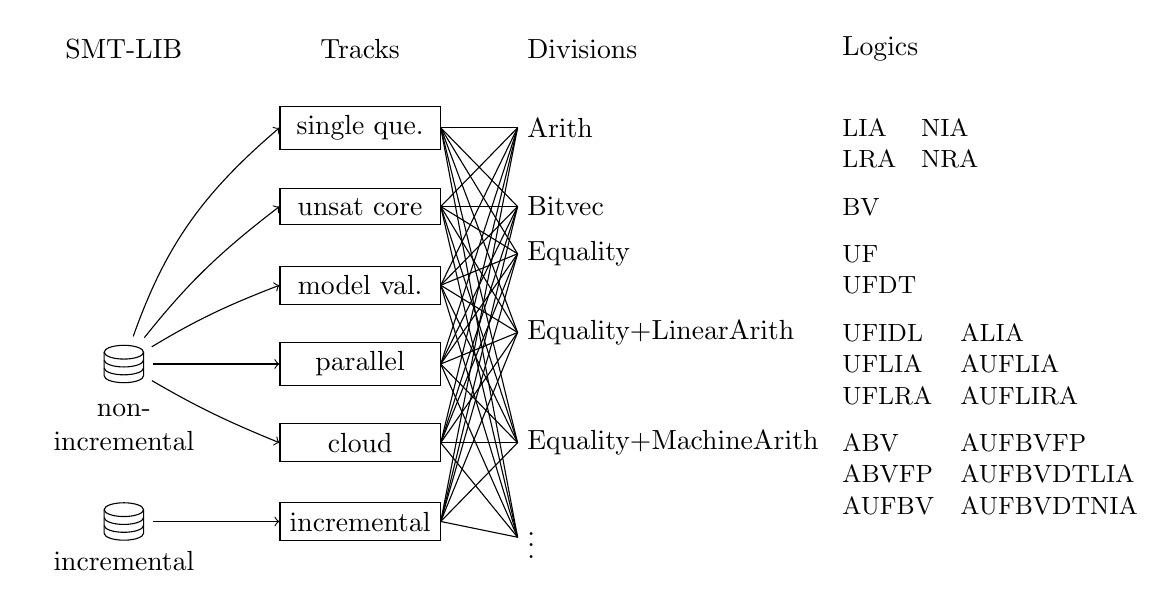
\begin{tikzpicture}
    \node at (0,6) {SMT-LIB};
    \node at (3,6) {Tracks};
    \node[anchor=west] at (5,6) {Divisions};
    \node[anchor=west] at (9,6) {Logics};

    \node[database,label=below:{\begin{tabular}{c}non-\\incremental\end{tabular}}] (nonincbench) at (0,2) {};
    \node[database,label=below:{incremental}] (incbench) at (0,0) {};

    \node[draw,text width=1.8cm,align=center](sq) at (3,5) {single que.};
    \node[draw,text width=1.8cm,align=center](uc) at (3,4) {unsat core};
    \node[draw,text width=1.8cm,align=center](mv) at (3,3) {model val.};
    \node[draw,text width=1.8cm,align=center](par) at (3,2) {parallel};
    \node[draw,text width=1.8cm,align=center](cloud) at (3,1) {cloud};
    \node[draw,text width=1.8cm,align=center](inc) at (3,0) {incremental};

    \node[anchor=west] (div1) at (5,5) {Arith};
    \node[anchor=west] at (9,5) {\small LIA};
    \node[anchor=west] at (9,4.6) {\small LRA};
    \node[anchor=west] at (10,5) {\small NIA};
    \node[anchor=west] at (10,4.6) {\small NRA};
    \node[anchor=west] (div2) at (5,4) {Bitvec};
    \node[anchor=west] at (9,4) {\small BV};
    \node[anchor=west] (div3) at (5,3.4) {Equality};
    \node[anchor=west] at (9,3.4) {\small UF};
    \node[anchor=west] at (9,3) {\small UFDT};
    \node[anchor=west] (div4) at (5,2.4) {Equality+LinearArith};
    \node[anchor=west] at (9,2.4) {\small UFIDL};
    \node[anchor=west] at (9,2) {\small UFLIA};
    \node[anchor=west] at (9,1.6) {\small UFLRA};
    \node[anchor=west] at (10.5,2.4) {\small ALIA};
    \node[anchor=west] at (10.5,2) {\small AUFLIA};
    \node[anchor=west] at (10.5,1.6) {\small AUFLIRA};
    \node[anchor=west] at (12.5,2) {$\hdots$};
    \node[anchor=west] (div5) at (5,1) {Equality+MachineArith};
    \node[anchor=west] at (9,1) {\small ABV};
    \node[anchor=west] at (9,.6) {\small ABVFP};
    \node[anchor=west] at (9,.2) {\small AUFBV};
    \node[anchor=west] at (10.5,1) {\small AUFBVFP};
    \node[anchor=west] at (10.5,.6) {\small AUFBVDTLIA};
    \node[anchor=west] at (10.5,.2) {\small AUFBVDTNIA};
    \node[anchor=west] at (12.5,1) {$\hdots$};
    \node[anchor=west] (div6)  at (5,-.2) {$\vdots$};

    \draw[->,shorten <=.3em] (nonincbench) to[bend left=15] (sq.west);
    \draw[->,shorten <=.3em] (nonincbench) to[bend left=7] (uc.west);
    \draw[->,shorten <=.3em] (nonincbench) to[bend left=5] (mv.west);
    \draw[->,shorten <=.3em] (nonincbench) to (par.west);
    \draw[->,shorten <=.3em] (nonincbench) to[bend right=4] (cloud.west);
    \draw[->,shorten <=.3em] (incbench) to (inc.west);

    \draw (sq.east) to (div1.west);
    \draw (sq.east) to (div2.west);
    \draw (sq.east) to (div3.west);
    \draw (sq.east) to (div4.west);
    \draw (sq.east) to (div5.west);
    \draw (sq.east) to (div6.west);

    \draw (uc.east) to (div1.west);
    \draw (uc.east) to (div2.west);
    \draw (uc.east) to (div3.west);
    \draw (uc.east) to (div4.west);
    \draw (uc.east) to (div5.west);
    \draw (uc.east) to (div6.west);

    \draw (mv.east) to (div1.west);
    \draw (mv.east) to (div2.west);
    \draw (mv.east) to (div3.west);
    \draw (mv.east) to (div4.west);
    \draw (mv.east) to (div5.west);
    \draw (mv.east) to (div6.west);

    \draw (cloud.east) to (div1.west);
    \draw (cloud.east) to (div2.west);
    \draw (cloud.east) to (div3.west);
    \draw (cloud.east) to (div4.west);
    \draw (cloud.east) to (div5.west);
    \draw (cloud.east) to (div6.west);

    \draw (par.east) to (div1.west);
    \draw (par.east) to (div2.west);
    \draw (par.east) to (div3.west);
    \draw (par.east) to (div4.west);
    \draw (par.east) to (div5.west);
    \draw (par.east) to (div6.west);

    \draw (inc.east) to (div1.west);
    \draw (inc.east) to (div2.west);
    \draw (inc.east) to (div3.west);
    \draw (inc.east) to (div4.west);
    \draw (inc.east) to (div5.west);
    \draw (inc.east) to (div6.west);
  \end{tikzpicture}

\end{frame}

\begin{frame}[fragile]{SMT-COMP Tracks (traditional)}
  \emph{Single Query (SQ) Track}
  \begin{itemize}
  \item Determine satisfiability of one problem
  \item Solver answers sat/unsat/unknown
  \end{itemize}
  \medskip

  \emph{Unsat Core Track}
  \begin{itemize}
  \item Find small unsatisfiable subset of input.
  \item Solver answers unsat + list of formulas.
  \end{itemize}
  \medskip

  \emph{Model Validation Track}
  \begin{itemize}
  \item Find a model for a satisfiable problem.
  \item Solver answers sat + value for each non-logical symbol.
  \end{itemize}
  \medskip

  \emph{Incremental Track}
  \begin{itemize}
  \item Solve many small problems interactively.
  \item Solver acks commands and answers sat/unsat for each check.
  \end{itemize}
\end{frame}

\begin{frame}[fragile]{SMT-COMP Tracks (experimental)}

  \emph{Model Validation}
  \begin{itemize}
    \item Division with quantifier-free floating-point logics
    \item Model validation with Dolmen (thanks to Gillaume Bury and Fran\c{c}ois
    Bobot)
  \end{itemize}
  \bigskip

  \emph{Cloud and Parallel Track} (sponsored by AWS, led by Mike Whalen)
  \begin{itemize}
  \item Solve a large problem over the cloud (or a big computer)
  \begin{itemize}
    \item 100 machines, 1600 cores, 6400 GB of memory (cloud)
    \item 64 cores, 256 GB of memory (parallel)
  \end{itemize}
  \item Solver answers sat/unsat/unknown
  \end{itemize}

  \pause\bigskip

  \emph{Proof Exhibition Track}
  \begin{itemize}
  \item Solver submitted together with a checker for unsatisfiability proofs
  \item No predefined format or checker
  \item No ranking
  \item Qualitative assessment
\end{itemize}

\medskip
\pause
  \emph{This year} the sat/unsat results from sound solvers in SQ were used to
  include benchmarks on the MV, UC and PE tracks.

\end{frame}


\begin{frame}{Tracks, Solvers, Divisions, and Benchmarks}
  Teams: 21 (+3)
  \bigskip

  \begin{tabular}{c|r@{}l|r@{}l|c}
    Track & \multicolumn{2}{c|}{Solvers} & \multicolumn{2}{c|}{Divisions}  & Benchmarks \\
    \hline
    Single Query  &  22&(+3)  & 19&(+1)  & 93\,945 \\
    Incremental &  8&(+1)   & 17&(+2)  & 22\,300   \\
    Unsat Core  &  6&(-1)   & 18&(+1)  & 57\,245  \\
    Model Validation  &  8&(+1)    &  7& (+ 1 exp.)  & 32\,766  \\
    Proof Exhibition  &  &4    &  & 18 exp.  & 57\,245  \\
    \hline
    Parallel &   4&(+1)      &   &14 exp.  & 400 \\
    Cloud & 4&(-1)      &  &14 exp.  & 400 \\

  \end{tabular}
  \bigskip

  Number in parenthesis shows changes from 2021
\end{frame}

\begin{frame}
  \frametitle{Participants}

  SMT-COMP 2022 participants rely on multiple reasoning frameworks:
  \begin{itemize}
  \item CDCL(T)
  \item mcSAT
  \item saturation
  \item automata
  \item finite domain
  \item CP
  \item local search
  \item besides wrappers extending the scope of existing solvers
  \end{itemize}

  \bigskip
  Six new solvers participated:
  \begin{itemize}
  \item NRA-LS   {\footnotesize (Liu et al.)}
  \item OSTRICH {\footnotesize (Chen et al.)}
  \item Yices-ismt {\footnotesize (Jia et al.)}
  \item Z3++ {\footnotesize (Cai et al.)}
  \item solsmt {\footnotesize (Reitwiessner and Soos)}
  \end{itemize}

\end{frame}

\section{Solver Presentation}


{
\begin{frame}
  \vspace*{-1pt}%
  \noindent\makebox[\textwidth]{%
    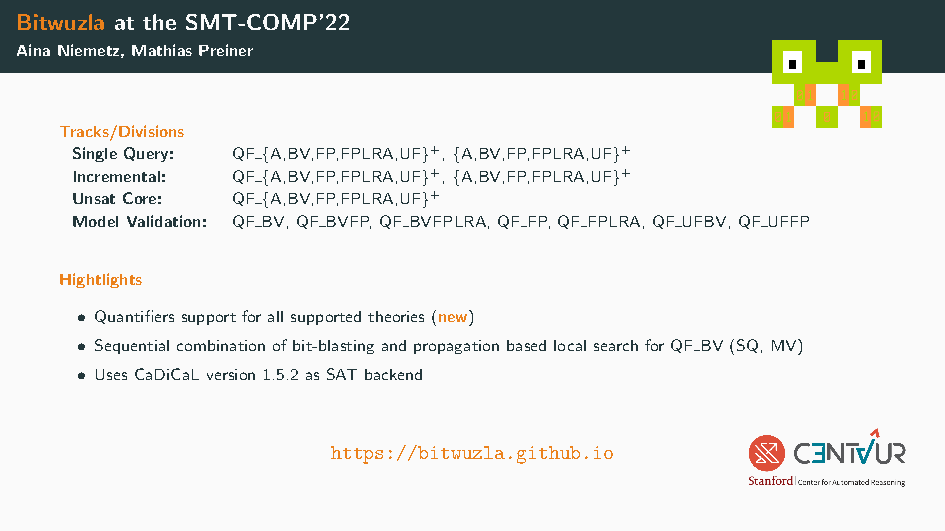
\includegraphics[height=\paperheight]{slide-bitwuzla.pdf}}
\end{frame}
}

{
\begin{frame}
  \vspace*{-1pt}%
  \noindent\makebox[\textwidth]{%
    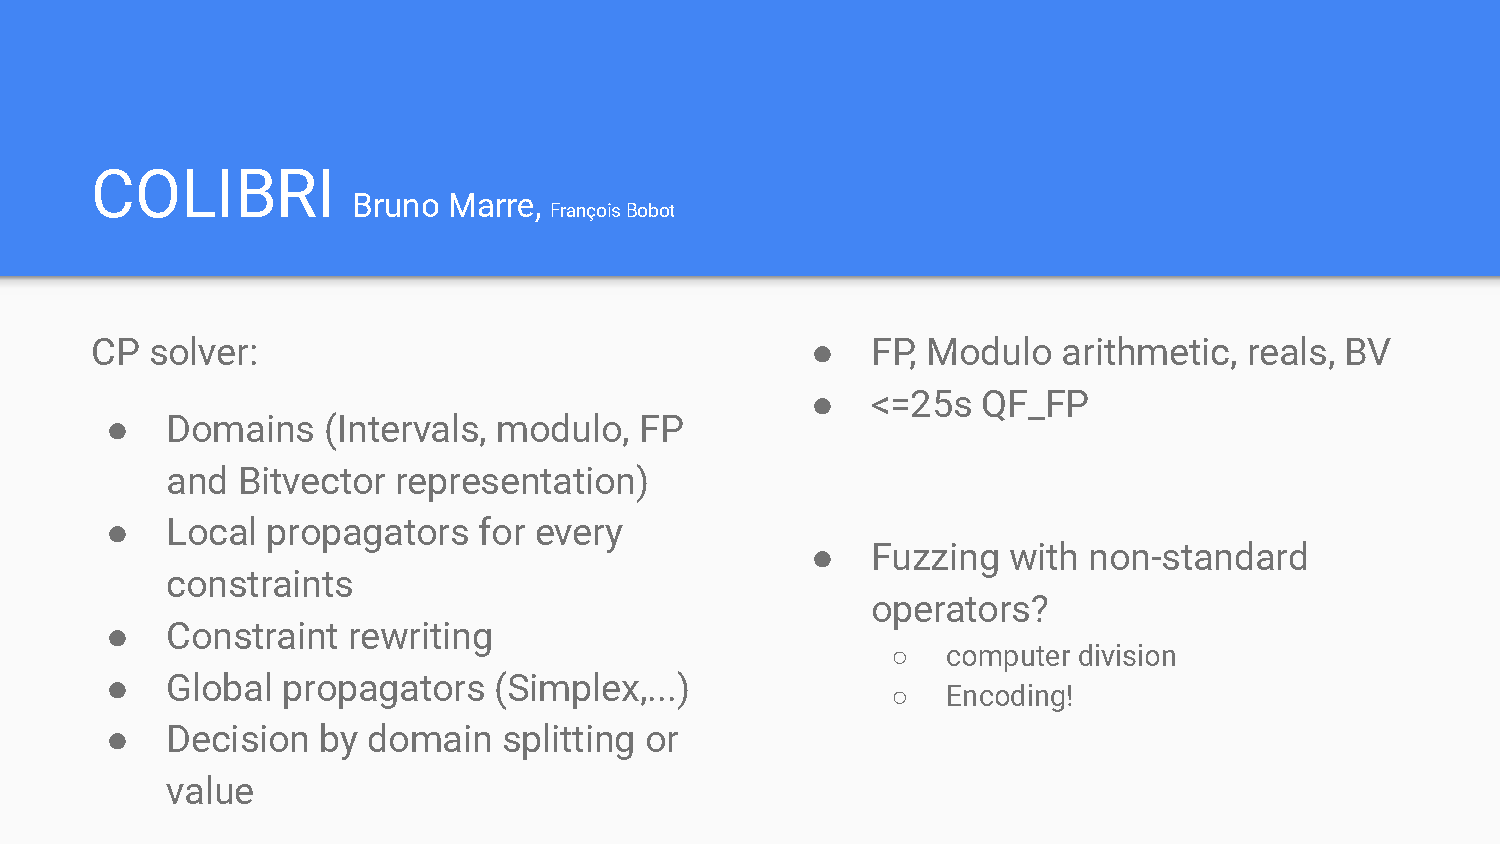
\includegraphics[height=\paperheight]{slide-colibri.pdf}}
\end{frame}
}

{
\begin{frame}
  \vspace*{-1pt}%
  \noindent\makebox[\textwidth]{%
    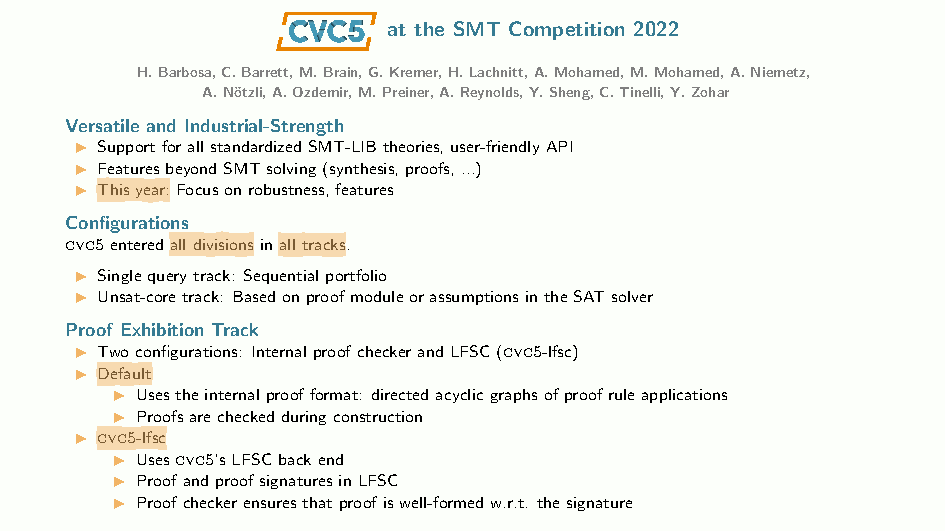
\includegraphics[height=\paperheight]{slide-cvc5.pdf}}
\end{frame}
}

{
\begin{frame}
  \vspace*{-1pt}%
  \noindent\makebox[\textwidth]{%
    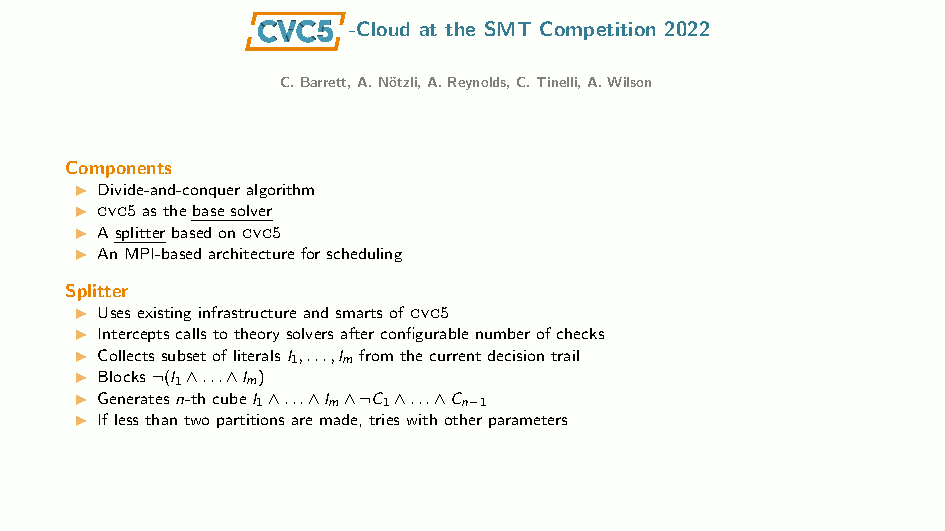
\includegraphics[height=\paperheight]{slide-cvc5-cloud.pdf}}
\end{frame}
}

{
\begin{frame}
  \vspace*{-1pt}%
  \noindent\makebox[\textwidth]{%
    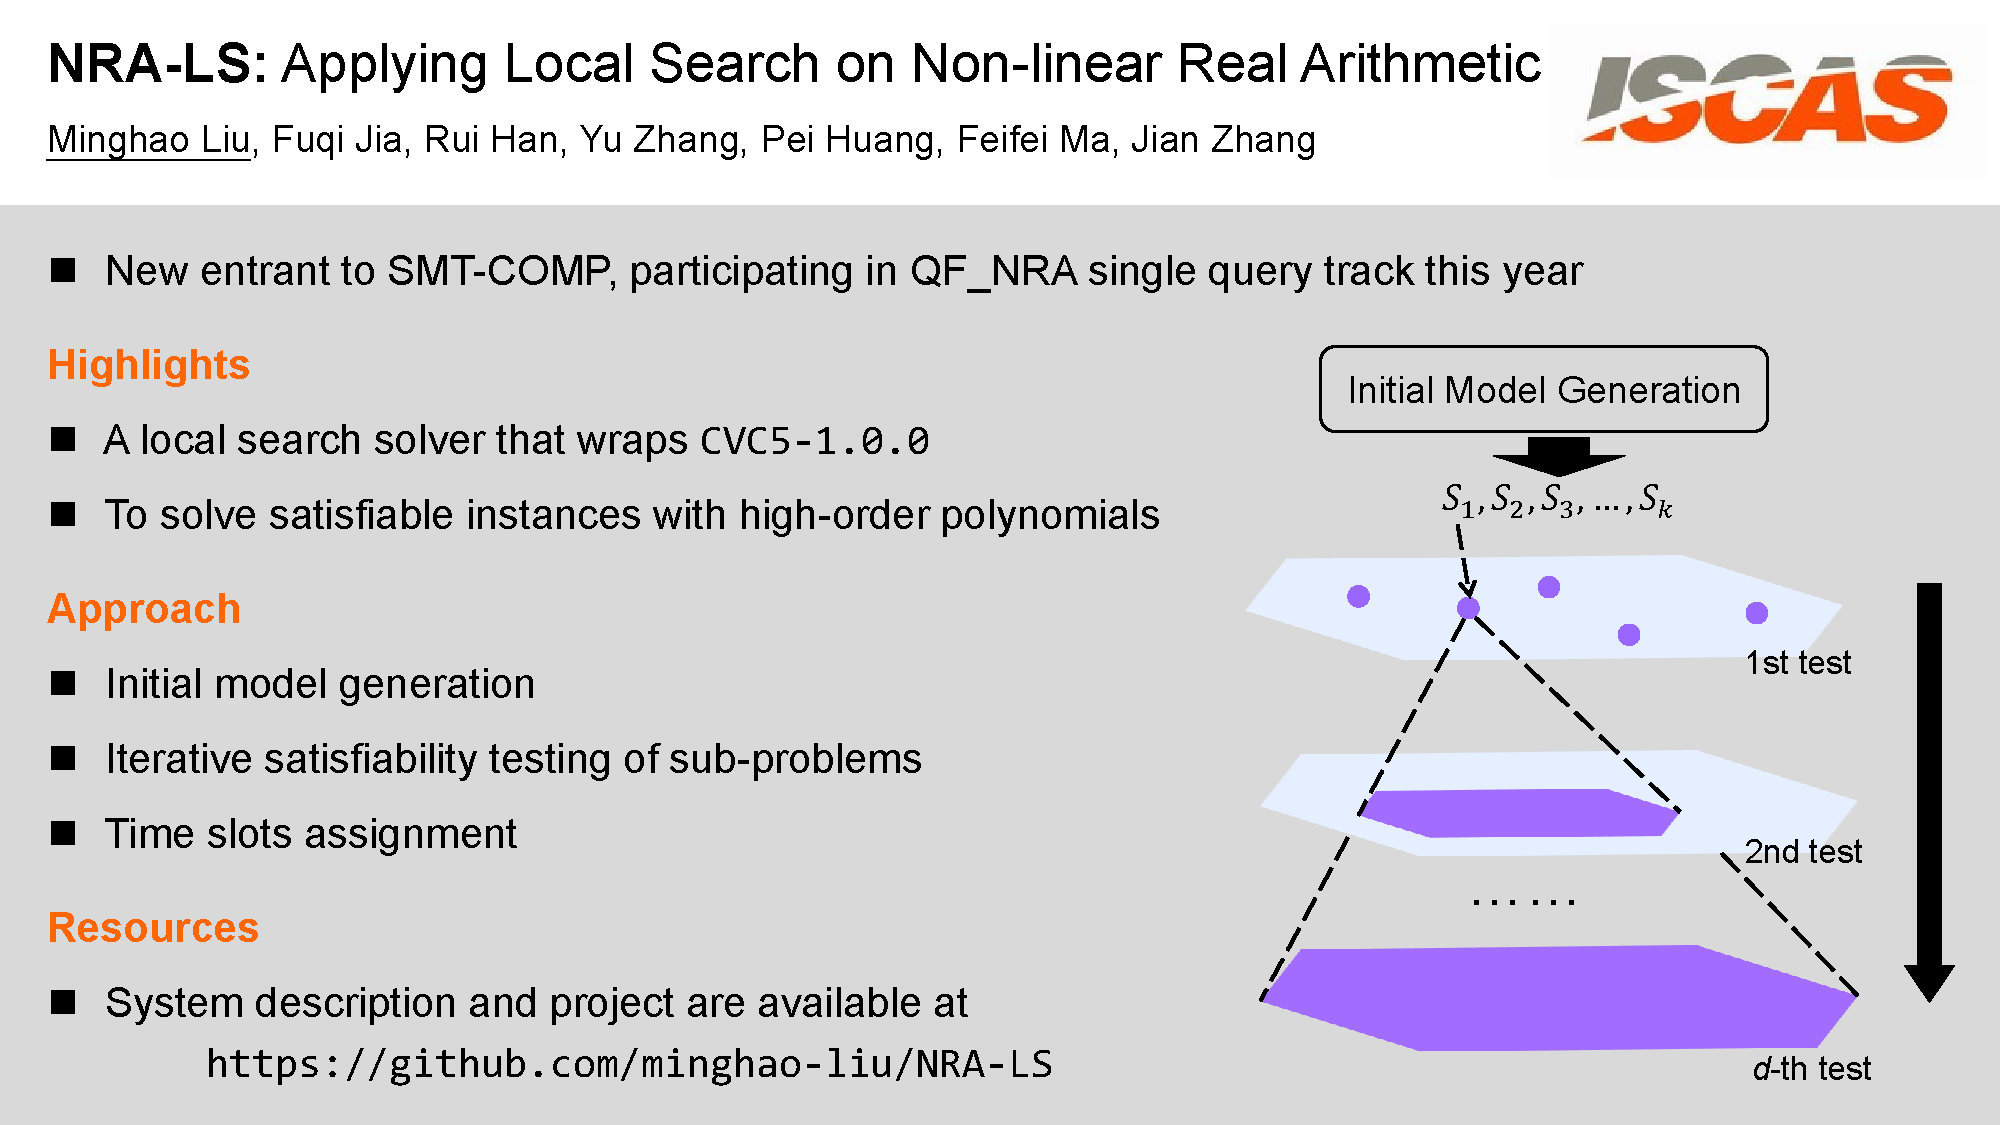
\includegraphics[height=\paperheight]{slide-nra-ls.pdf}}
\end{frame}
}

{
\begin{frame}
  \vspace*{-1pt}%
  \noindent\makebox[\textwidth]{%
    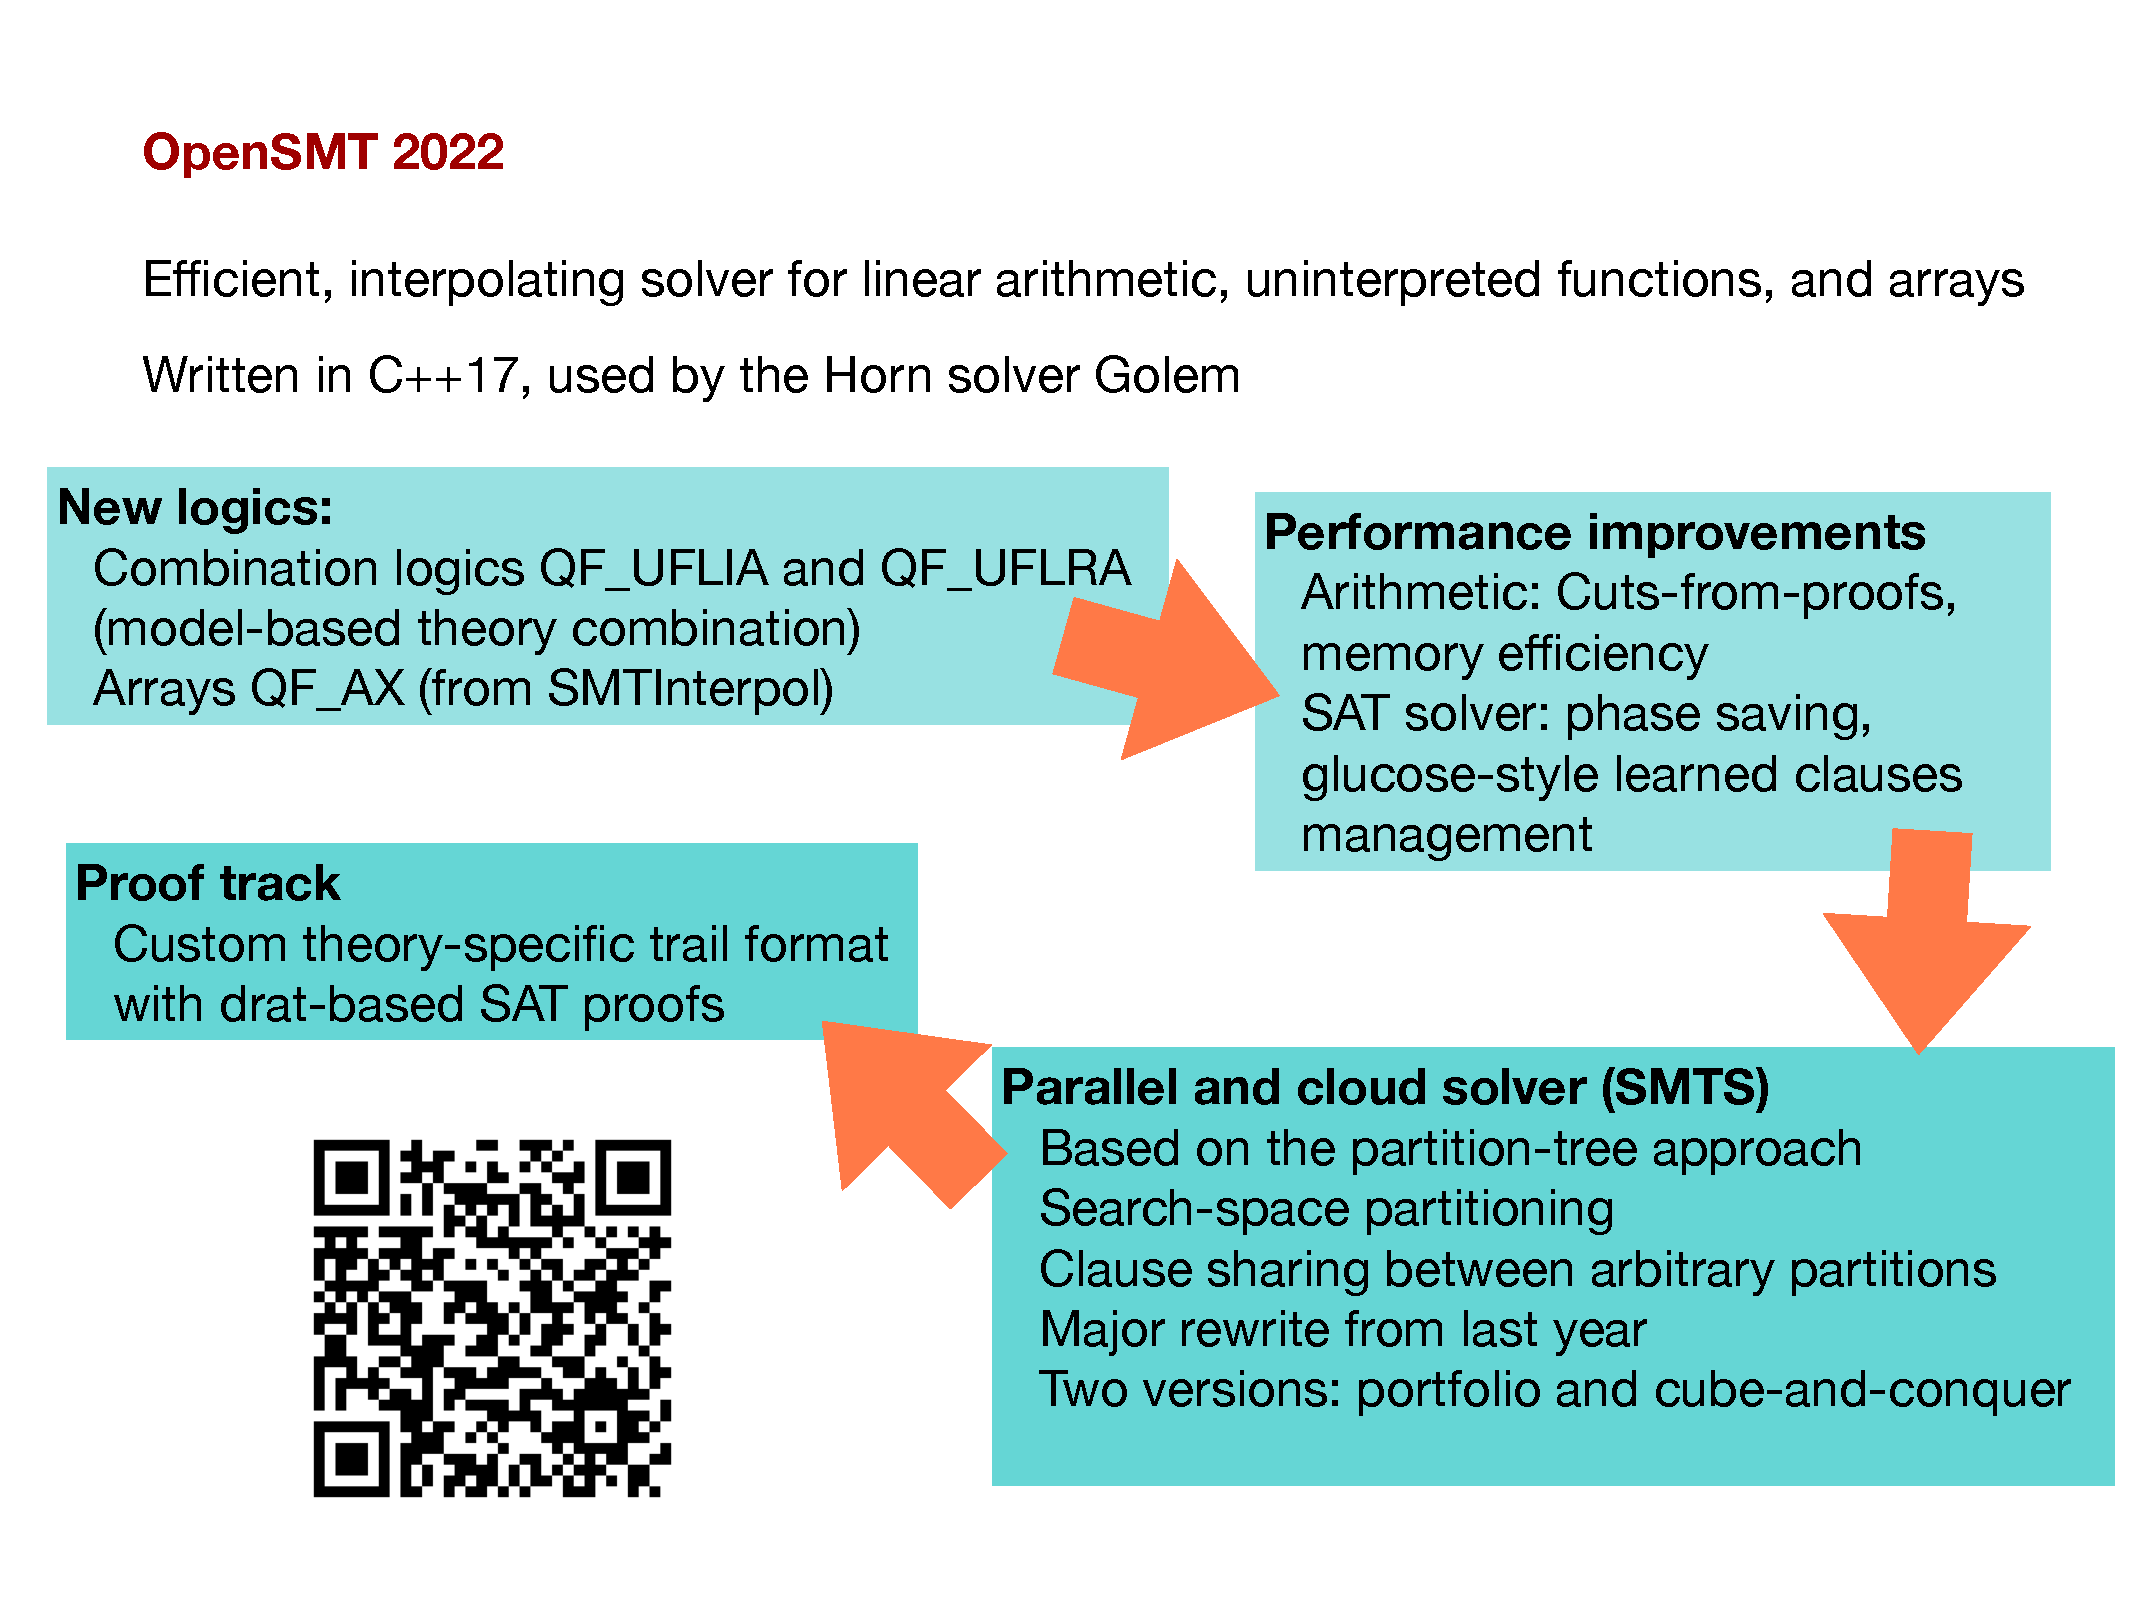
\includegraphics[height=\paperheight]{slide-opensmt.pdf}}
\end{frame}
}

{
\begin{frame}
  \vspace*{-1pt}%
  \noindent\makebox[\textwidth]{%
    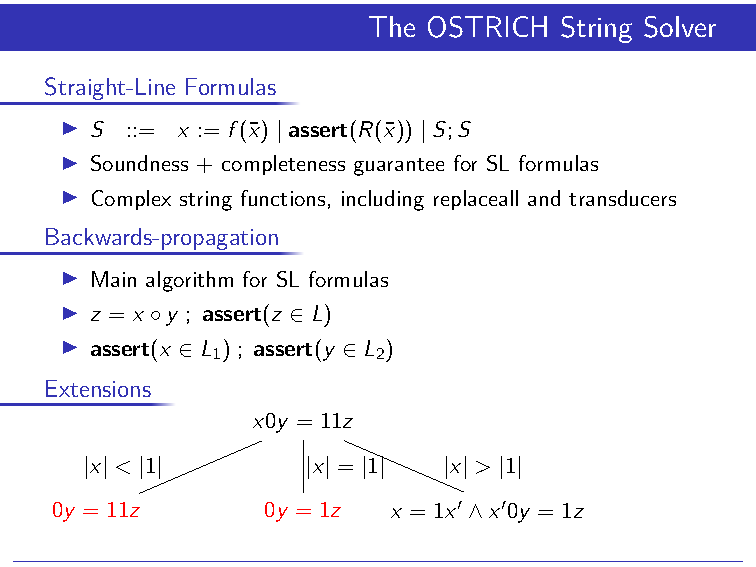
\includegraphics[height=\paperheight]{slide-ostrich.pdf}}
\end{frame}
}

{
\begin{frame}
  \vspace*{-1pt}%
  \noindent\makebox[\textwidth]{%
    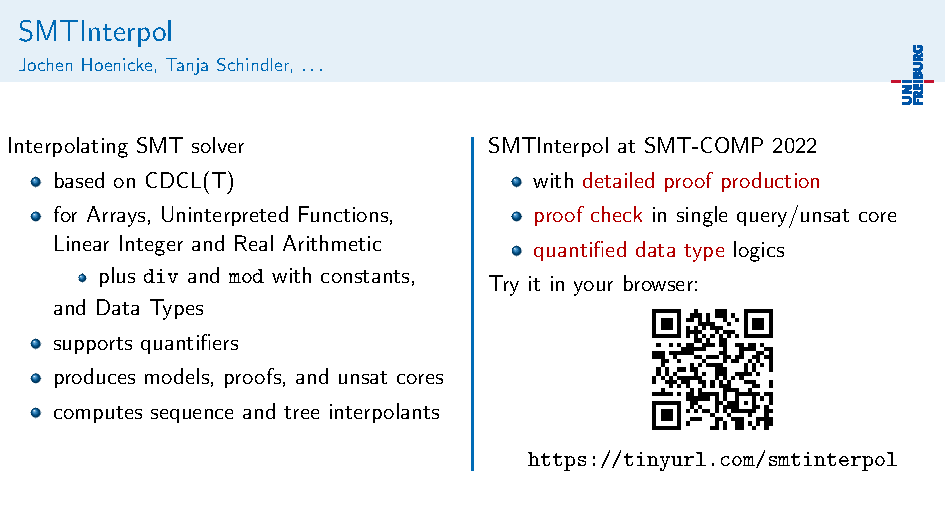
\includegraphics[height=\paperheight]{slide-smtinterpol.pdf}}
\end{frame}
}

{
\begin{frame}
  \vspace*{-1pt}%
  \noindent\makebox[\textwidth]{%
    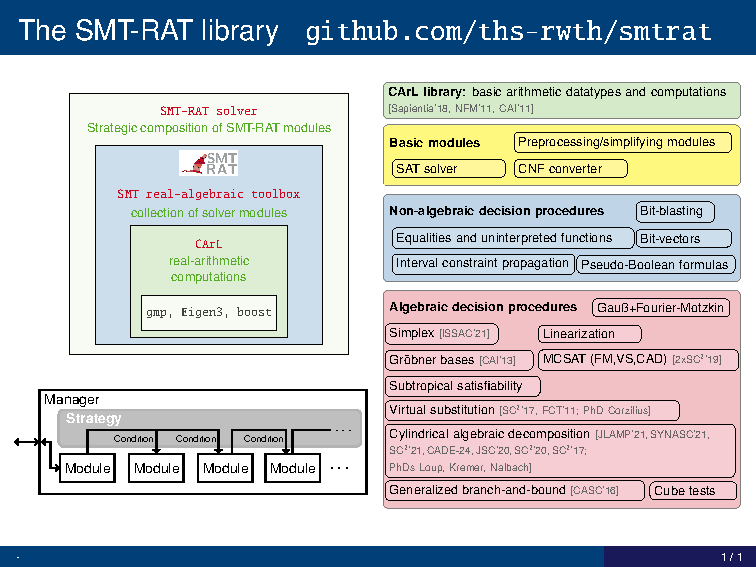
\includegraphics[height=\paperheight]{slide-smtrat.pdf}}
\end{frame}
}

{
\begin{frame}
  \vspace*{-1pt}%
  \noindent\makebox[\textwidth]{%
    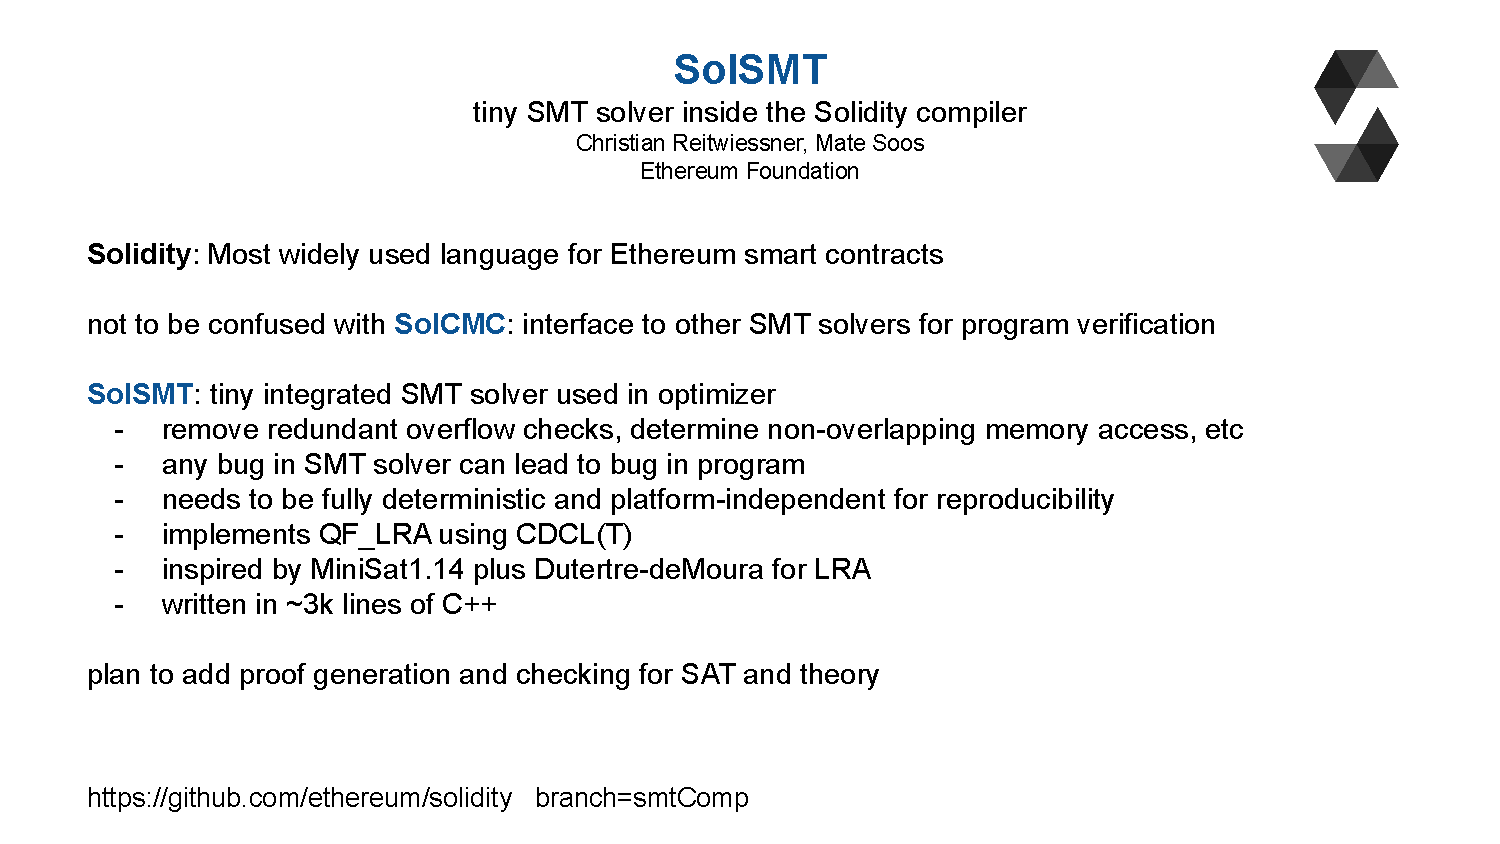
\includegraphics[height=\paperheight]{slide-solsmt.pdf}}
\end{frame}
}

{
\begin{frame}
  \vspace*{-1pt}%
  \noindent\makebox[\textwidth]{%
    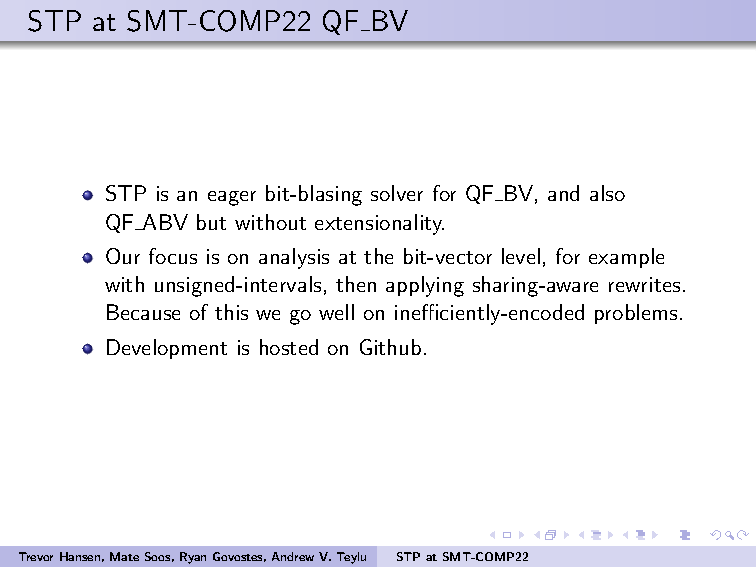
\includegraphics[height=\paperheight]{slide-stp.pdf}}
\end{frame}
}

{
\begin{frame}
  \vspace*{-1pt}%
  \noindent\makebox[\textwidth]{%
    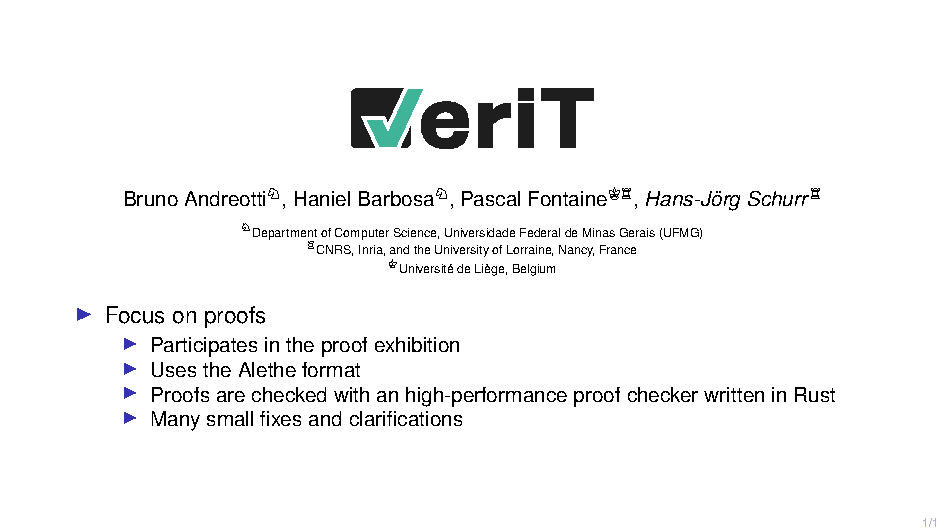
\includegraphics[height=\paperheight]{slide-verit.pdf}}
\end{frame}
}

{
\begin{frame}
  \vspace*{-1pt}%
  \noindent\makebox[\textwidth]{%
    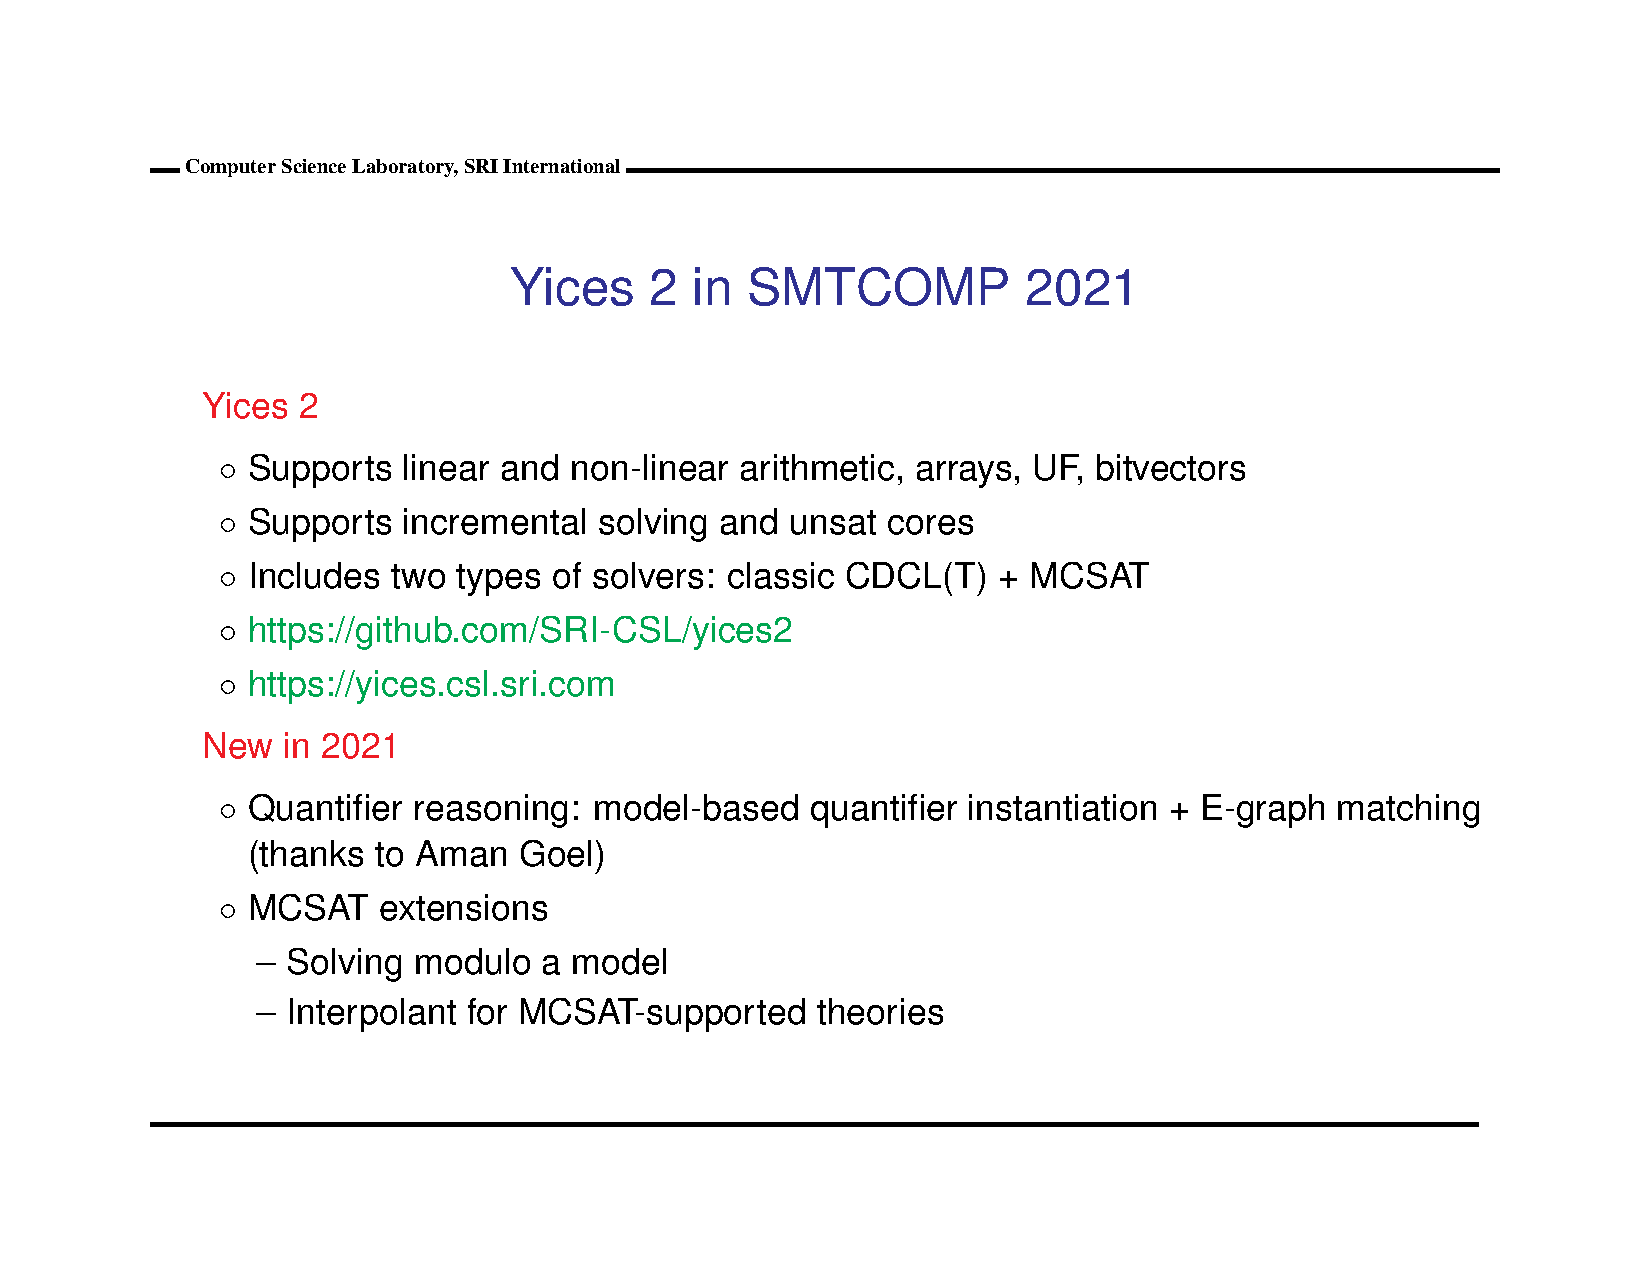
\includegraphics[height=\paperheight]{slide-yices.pdf}}
\end{frame}
}

{
\begin{frame}
  \vspace*{-1pt}%
  \noindent\makebox[\textwidth]{%
    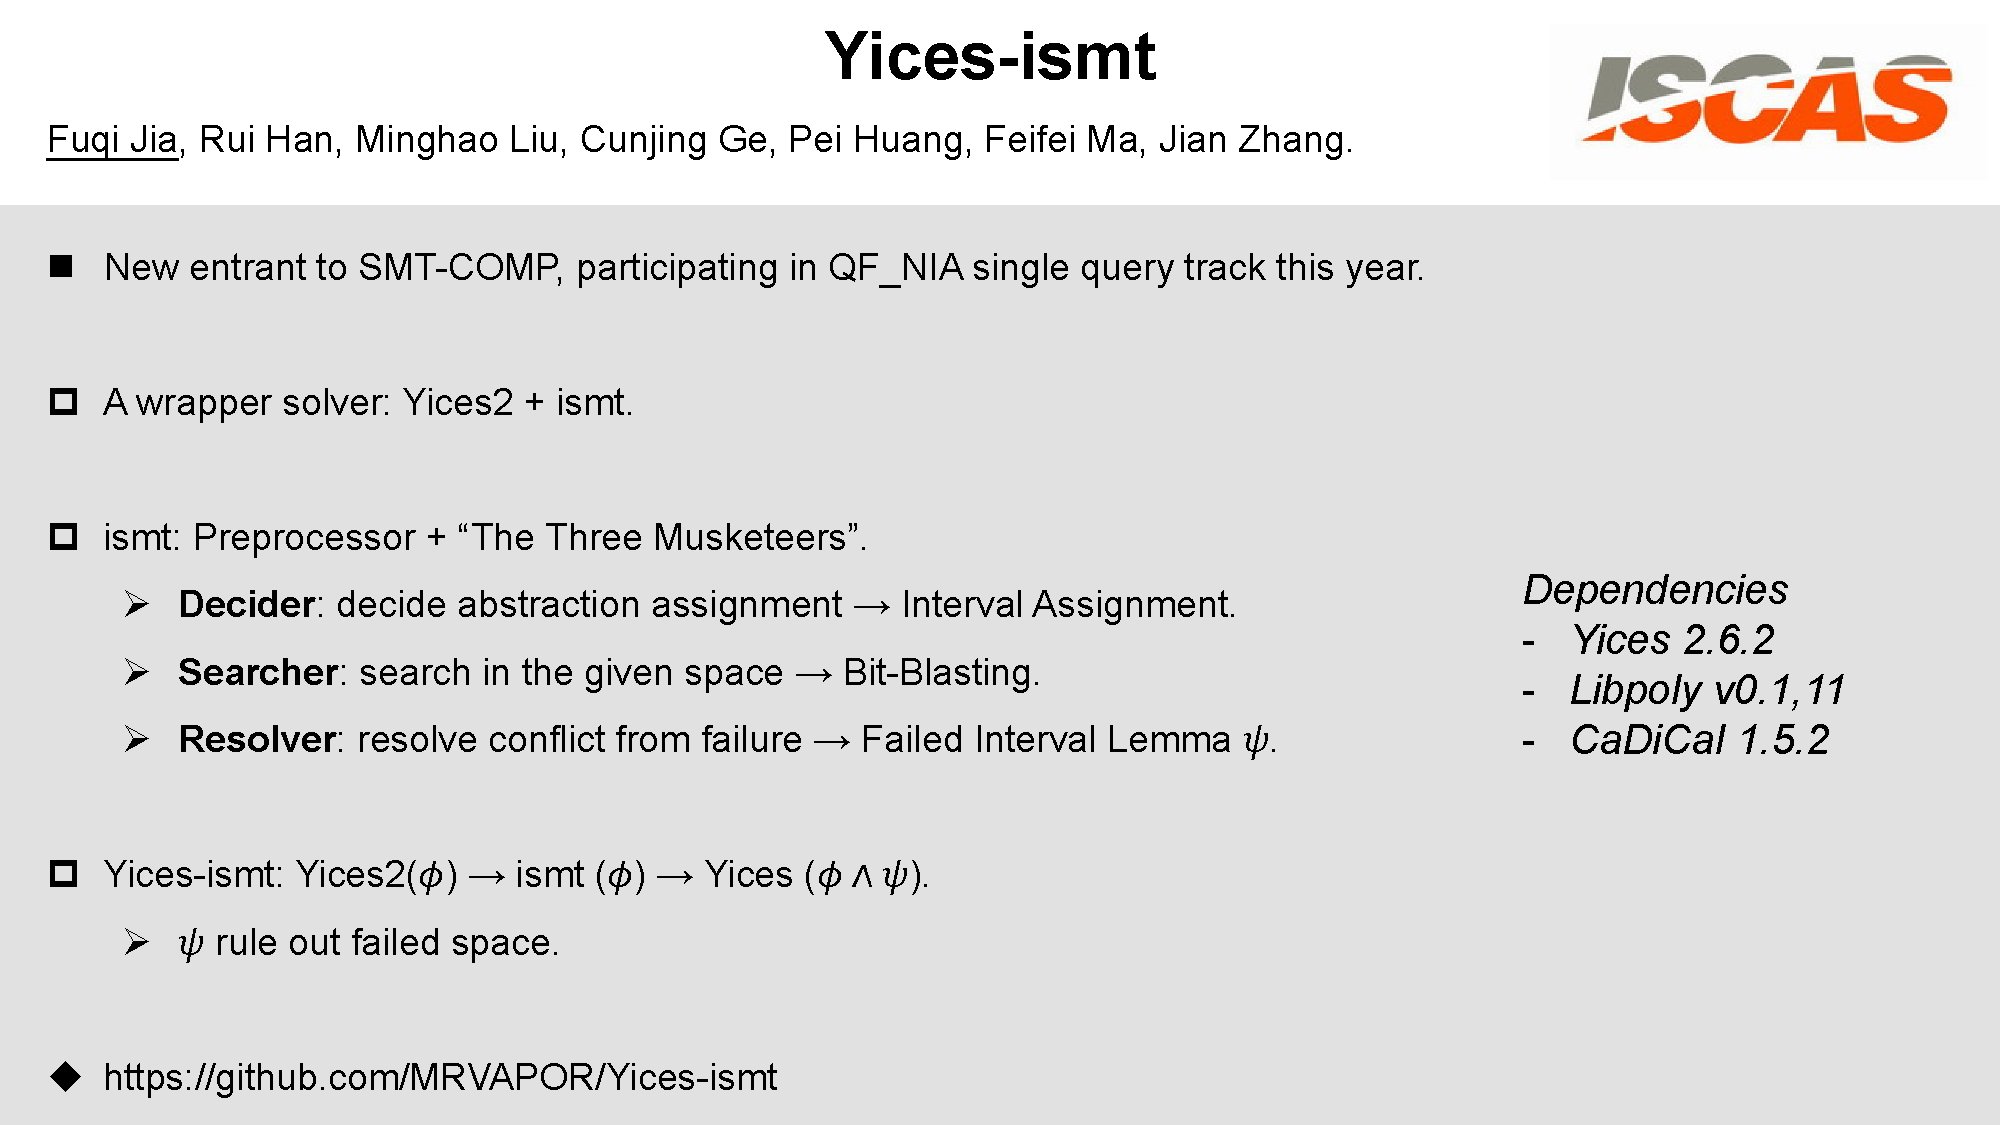
\includegraphics[height=\paperheight]{slide-yices-ismt.pdf}}
\end{frame}
}

{
\begin{frame}
  \vspace*{-1pt}%
  \noindent\makebox[\textwidth]{%
    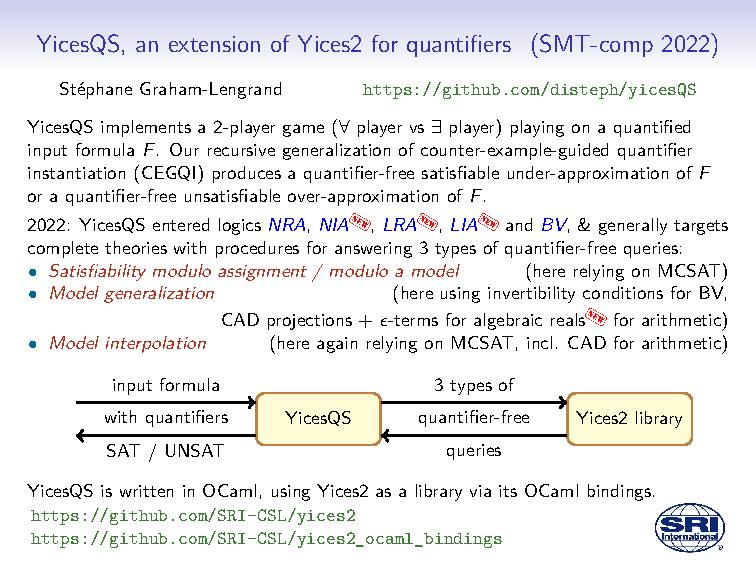
\includegraphics[height=\paperheight]{slide-yices-qs.pdf}}
\end{frame}
}

{
\begin{frame}
  \vspace*{-1pt}%
  \noindent\makebox[\textwidth]{%
    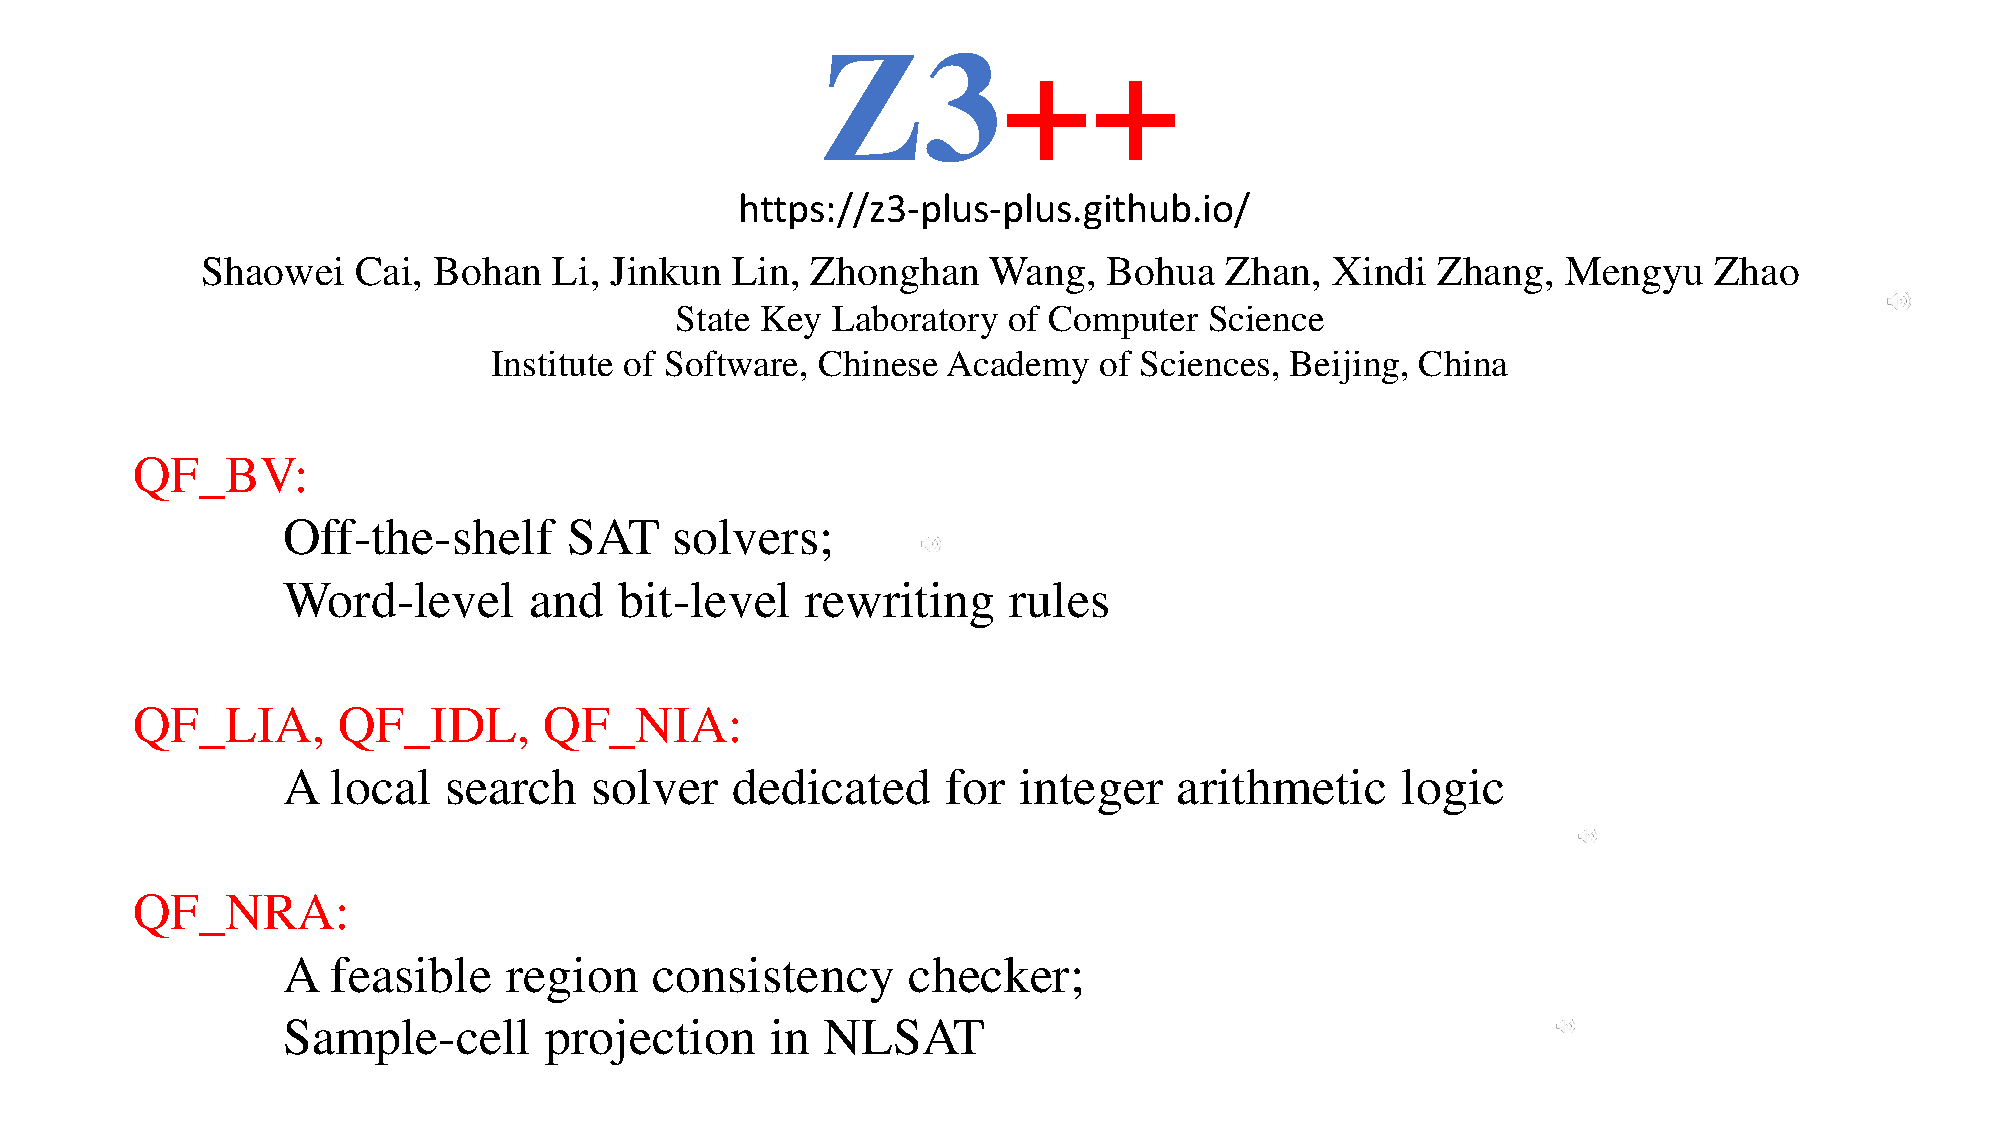
\includegraphics[height=\paperheight]{slide-z3pp.pdf}}
\end{frame}
}

{
  \begin{frame}
    \frametitle{Other participants}
    \begin{itemize}
      \item Q3B
      \vitem SMT-RAT
      \vitem SMTS
      \vitem UltimateEliminatior+MathSAT
      \vitem Vampire
      \vitem Z3str4
    \end{itemize}
  \end{frame}
}

\begin{frame}
  \frametitle{Non-Competitive Solvers}

  Submitted by organisers
  \begin{itemize}
  \item z3-4.8.17
  \item MathSAT 5.6.8
  \item Best solvers, per division, from previous years (23 Solvers)
  \end{itemize}
  \bigskip

  Submitted by participants
  \begin{itemize}
  \item Fixed solvers (OpenSMT, STP, Yices-ismt, Z3++,smtinterpol)
  \end{itemize}
\end{frame}

\begin{frame}{Scoring}
  Computing scores:
  \begin{itemize}
  \item \emph{Single Query/Parallel/Cloud}: number of solved \emph{instances}
  \item \emph{Incremental}: number of solved \emph{queries}
  \item \emph{Unsat Core}: number of top-level assertions \emph{removed}
  \item \emph{Model Validation}: number of solved instances with correct \emph{models}
  \end{itemize}

  \bigskip
  Error scores:
  \begin{itemize}
  \item \emph{All Tracks}: given for sat reply for unsat instance, or vice versa
  \item \emph{Unsat Core}: given if returned core is satisfiable.
  \item \emph{Model Validation}: given if given model evaluates formula to \emph{false}
  \end{itemize}
  Error scores are draconian.
\end{frame}

\begin{frame}{Score and Ranking}
  In each track we collect different scores:
  \begin{itemize}
  \item \emph{Sequential score} (SQ, UC, MV): all time limits apply to cpu time
  \item \emph{Parallel score} (all): all time limits apply to wallclock time
  \item \emph{SAT score} (SQ): parallel score for \emph{satisfiable} instances
  \item \emph{UNSAT score} (SQ): parallel score for \emph{unsatisfiable} instances
  \item \emph{24s} (SQ): parallel score with time limit of \emph{24s}
  \end{itemize}
  \bigskip

  Division ranking (for each score)
  \begin{itemize}
  \item For each division, one winner is declared
  \end{itemize}

  \bigskip

  Two competition-wide rankings (for each score)
  \begin{itemize}
  \item \emph{Biggest lead}: division winner with most score difference to second place
  \item \emph{Largest contribution}: improvement each solver provided to a virtual best solver
  \end{itemize}

\end{frame}

\begin{frame}{Division Winners}
  \pause
  \emph{Single Query, sequential score}
  \begin{itemize}
  \item \emph{Bitwuzla}: {\small FPArith, QF\_Bitvec, QF\_Equality+Bitvec, QF\_FPArith}

  \item \emph{cvc5}: \begin{minipage}{.8\textwidth}\raggedright \tiny Arith,
    Bitvec, Equality, Equality+LinearArith, Equality+MachineArith,
    Equality+NonLinearArith, QF\_Datatypes, QF\_Equality+NonLinearArith, QF\_NonLinearIntArith, QF\_NonLinearRealArith, QF\_Strings\end{minipage}

  \item \emph{OpenSMT}: {\small QF\_LinearIntArith}

  \item \emph{SMTInterpol}: {\small QF\_Equality+LinearArith}

  \item \emph{Yices2}: {\small QF\_Equality, QF\_LinearRealArith}
  \end{itemize}

  \medskip

  \pause
  \emph{Unsat Core}
  \begin{itemize}
\item \emph{cvc5}: Arith, Bitvec, Equality+LinearArith, Equality+MachineArith,Equality+NonLinearArith,Equality(Seq), QF\_Datatypes
\item \emph{Vampire}: Equality(Par)
\item \emph{Bitwuzla}: QF\_EqualityBitvec, QF\_FPArith
\item \emph{Yices2}: QF\_Bitvec, QF\_Equality+LinearArith, QF\_Equality, QF\_LinearIntArith, QF\_LinearRealArith
\item \emph{SMTInterpol}: QF\_Equality+NonLinearArith
\item \emph{UltimateEliminator+MathSAT}: FPArith

  \end{itemize}

\end{frame}

\begin{frame}{Division Winners}
  \emph{Incremental}
  \begin{itemize}
\item \emph{cvc5}: Arith, Bitvec, Equality+LinearArith,EqualityNonLinearArith,Equality
\item \emph{UltimateEliminator+MathSAT}: Equality+MachineArith
\item \emph{Bitwuzla}: FPArith, QF\_FPArith
\item \emph{Yices2}: QF\_Bitvec, QF\_Equality+Bitvec, QF\_Equality, QF\_LinearIntArith
\item \emph{SMTInterpol}: QF\_Equality+LinearArith, QF\_Equality+NonLinearArith, QF\_NonLinearIntArith
\item \emph{OpenSMT}: QF\_LinearRealArith
  \end{itemize}
  \medskip

  \pause
  \emph{Model Validation (competitive only)}
  \begin{itemize}
\item \emph{Bitwuzla}: QF\_Bitvec, QF\_Equality+Bitvec,
\item \emph{smtinterpol}: QF\_Equality+LinearArith
\item \emph{Yices2}: QF\_Equality
\item \emph{Z3++}: QF\_LinearIntArith
\item \emph{OpenSMT}: QF\_LinearRealArith

\item experimental: QF\_FPArith : Bitwuzla, cvc5

  \end{itemize}
\end{frame}

\begin{frame}{Largest contribution}
  \begin{tabular}{r|c@{}lc@{}lc@{}l}
    &\textcolor{gold}{\textbf{1st Place}} &&
    \textcolor{silver}{\textbf{2nd Place}} &&
    \textcolor{bronze}{\textbf{3rd Place}}\\
    \hline
    \emph{Single Query}\\
    seq & cvc5&{\tiny(Eq+MA)} & YicesQS&{\tiny(Arith)} & Bitwuzla&{\tiny(FPArith)} \\
    par & cvc5&{\tiny(Eq+MA)} & YicesQS&{\tiny(Arith)} & Bitwuzla&{\tiny(FPArith)} \\
    sat & cvc5&{\tiny(Eq+LA)} & YicesQS&{\tiny(Arith)} & Bitwuzla&{\tiny(FPArith)} \\
    unsat & cvc5&{\tiny(Eq+MA)} & Z3++&{\tiny(QF\_NonLIA)} & OSTRICH&{\tiny(QF\_Strings)}\\
    24 &  Vampire&{\tiny(Eq+NA)} & Vampire&{\tiny(Equality)} & Yices2&{\tiny(QF\_LinIA)}\\[3pt]
    \pause
    \emph{Incremental}\\
    par & cvc5&{\tiny(Eq+NA)} &Yices2&{\tiny(QF\_Eq+LA)}
    &SMTInterpol&{\tiny(QF\_Eq+NA)}\\[3pt]
    \pause

    \emph{Unsat Core}\\
    seq & cvc5&{\tiny(Eq+LA)} &
    Bitwuzla&{\tiny(QF\_Eq+Bitvec)}\\

    par &  cvc5&{\tiny(Eq+NA)}&
    Bitwuzla&{\tiny(QF\_Eq+Bitvec)}\\
\\[3pt]
    \pause
    \emph{Model Validation}\\
    seq &  Z3++&{\tiny(QF\_LinIA)} & Bitwuzla&{\tiny(QF\_Bitvec)}
        & smtinterpol&{\tiny(QF\_Eq+LIA)}\\
    par &  Z3++&{\tiny(QF\_LinIA)} & Bitwuzla&{\tiny(QF\_Bitvec)}
        & smtinterpol&{\tiny(QF\_Eq+LIA)}\\
  \end{tabular}
\end{frame}


\begin{frame}{Biggest Lead}
  \begin{tabular}{r|c@{}lc@{}lc@{}l}
    &\textcolor{gold}{\textbf{1st Place}} &&
    \textcolor{silver}{\textbf{2nd Place}} &&
    \textcolor{bronze}{\textbf{3rd Place}}\\
    \hline
    \emph{Single Query}\\
    seq & cvc5&{\tiny(QF\_DT)} & Bitwuzla&{\tiny(FPArith)} & Yices2&{\tiny(QF\_LinRA)} \\
    par & cvc5&{\tiny(QF\_DT)} & Bitwuzla&{\tiny(FPArith)} & Yices2&{\tiny(QF\_LinRA)} \\
    sat & cvc5&{\tiny(QF\_DT)} & Bitwuzla&{\tiny(FPArith)} & Z3++&{\tiny(QF\_NonRA)} \\
    unsat & cvc5&{\tiny(QF\_DT)} & Z3++&{\tiny(QF\_NonIA)} & Bitwuzla&{\tiny(FPArith)} \\
    24 &  cvc5&{\tiny(Eq+MA)} & smtinterpol&{\tiny(QF\_DT)} & Vampire&{\tiny(Equality)}\\[3pt]
    \pause
    \emph{Incremental}\\
    par & SMTInterpol&{\tiny(QF\_NIA)}
    &Yices2&{\tiny(QF\_LinIA)} & cvc5&{\tiny(Eq+NonLA)} \\[3pt]
    \pause
    \emph{Unsat Core}\\
    seq & cvc5&{\tiny(Eq+MA)} &    Yices2&{\tiny(QF\_Eq+LA)} &    smtinterpol&{\tiny(QF\_Eq+NA)} \\
    par & cvc5&{\tiny(Eq+MA)} &    Yices2&{\tiny(QF\_Eq+LA)} &    smtinterpol&{\tiny(QF\_Eq+NA)} \\
    \pause
    \emph{Model Validation}\\
    seq &  Z3++&{\tiny(QF\_LinIA)} & smtinterpol&{\tiny(QF\_LinA)}        & OpenSMT&{\tiny(QF\_LinRA)} \\
    par &  Z3++&{\tiny(QF\_LinIA)} & smtinterpol&{\tiny(QF\_LinA)}        & OpenSMT&{\tiny(QF\_LinRA)} \\
  \end{tabular}
\end{frame}

\begin{frame}{Checking Disagreements}

  \begin{itemize}
  \item  111\,451 instances of 391\,363 have no status

  \vitem Only 18 benchmarks with disagreements (AUFDTLIA, QF\_NIA)

  \vitem We manually resolved the disagreements
  \begin{itemize}
    \item Authors confirmed solver unsoundness
    \item Sound solvers agreed on result
  \end{itemize}

  \vitem We had only three solvers with soundness issues: SMTIinterpol, Z3++,
  yices-ismt
  \begin{itemize}
    \item Down from 10 last year
    \pause
    {\tiny (but note that this may be because of our issue with ignoring most of the
    new benchmarks in the selection)}


  \end{itemize}
  \end{itemize}
\end{frame}

\begin{frame}{Plans for SMT-COMP 2022}
  \begin{itemize}
    \item Move to Dolmen as single model validator

      \vitem Dolmen worked well in QF\_FP (minor issue with empty output, simple
      to fix)
      \vitem pysmt timed out in two cases (locally with more time one of them
      succeeded)
      \vitem pysmt could not understand the model in 9 cases
      \vitem Dolmen is easy to extend to new theories
      \vitem Easy to integrate with correct-by-construction code extracted from
      Coq
      \vitem Should be more efficient for handling function call

  \end{itemize}


\end{frame}

\begin{frame}{Plans for SMT-COMP 2022}
  \begin{itemize}
    \item Proof \textit{validation} track

      \vitem Hopefully proof exhibition this year will help

      \vitem We have to analyze the data still
      \begin{itemize}
        \item Job only finished last week (took 18 days to run)
        \item 830gb
      \end{itemize}

  \end{itemize}


\end{frame}

\begin{frame}{SMT-COMP organizing committee}
  Three people organize the SMT-COMP.  In 2022:
  \begin{itemize}
  \item Haniel Barbosa
  \item Jochen Hoenicke
  \item Fran\c{c}ois Bobot
  \end{itemize}

  Both Haniel and Jochen have been organizers for three-years. One of them
  should be replaced.
  \bigskip

  We need a successor for next year's competition.
  Contact us if you would like to volunteer!
\end{frame}


\begin{frame}{Acknowledgements}
  \begin{itemize}
    \item \emph{Andrea Micheli}: pysmt
    \item \emph{Guillaume Bury}: Model Validator
    \item \emph{Clark Barrett, Pascal Fontaine, Aina Niemetz, Mathias Preiner, Hans-Jörg Schurr}: SMT-LIB benchmarks
    \item \emph{Aaron Stump}: StarExec support
    \item \emph{Mike Whalen and team}: Cloud/Parallel Track
  \end{itemize}
  \bigskip

  \begin{columns}
    \begin{column}{.3\textwidth}
      
\includegraphics[width=\textwidth]{starlogo}
    \end{column}
    \begin{column}{.17\textwidth}
      
\includegraphics[width=\textwidth]{powered-by-aws}
    \end{column}
  \end{columns}
\end{frame}

\begin{frame}[shrink=0.95]{Benchmark contributors}
  In 2022 \emph{new benchmarks} were contributed by:

  \small
  \begin{itemize}
    \item  Alex Coffin
    \item  Alex Ozdemir
    \item  Ali Uncu, James Davenport and Matthew England
    \item  Bohan Li
    \item  Elizabeth Polgreen
    \item  Fuqi Jia
    \item  Johann-Tobias Aaron and Raphael Schäg
    \item  Matthew England and Miguel Del Rio Almajano
    \item  Nicolas Amat
    \item  Yannick Moy
    \item  Yoni Zohar
  \end{itemize}
\end{frame}

\begin{frame}

  \begin{center}
    \Large\emph{Thanks}
  \end{center}

  \begin{center}
    to all participants
  \end{center}

  \bigskip
  \pause


  \begin{center}
    and to you for listening
  \end{center}

\end{frame}

\end{document}
